\section{Cryptography, Practical Optimizations, and Performance}
pBFT resolves cryptographic latency bottlenecks by reserving expensive public-key signatures (such as RSA) exclusively for critical operational transitions like view changes. In the normal case, it employs symmetric-key cryptography \textbf{Message Authentication Codes (MACs)} for the overwhelming majority of interactions, which perform orders of magnitude faster.

Additionally, it optimizes data transmission overhead by instructing only one designated replica to send the complete response payload back to the client, while the remaining nodes transmit only small cryptographic digests. For high-demand environments, pBFT utilizes request batching within a single consensus sequence and enables a fast path for read-only operations.

\subsection{Byzantine File System (BFS) Architecture}
To empirically demonstrate the "practical" value of pBFT, the authors developed a replication library upon which they implemented the Byzantine-Fault-tolerant File System (BFS). This filesystem supports the standard NFS V2 network protocol transparently, requiring no modifications to either the client or the original kernel server.

\begin{figure}[h!]
\centering
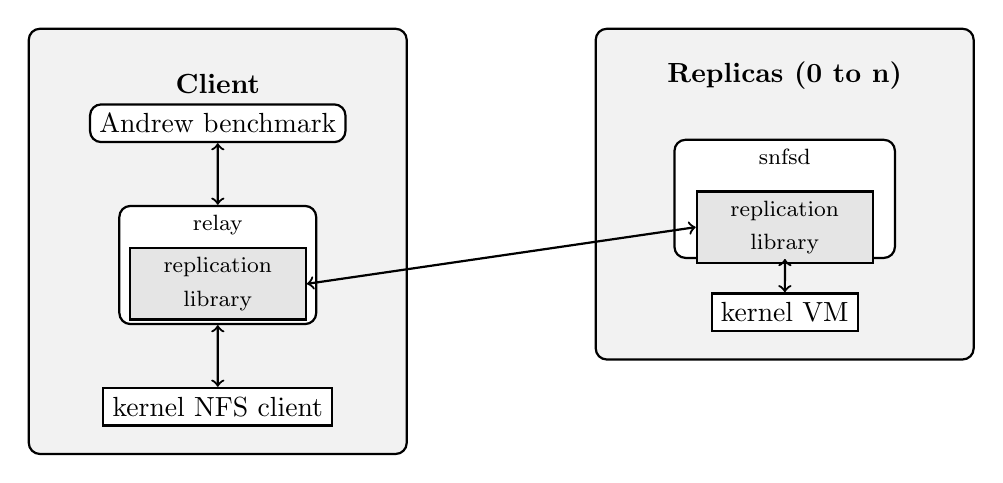
\begin{tikzpicture}[xscale=1.2, yscale=1.2, thick]
    % Client
    \draw[rounded corners, fill=black!5] (0,0) rectangle (4,4.5) node[pos=0.5, yshift=2.0cm] {\textbf{Client}};
    \node[draw, rounded corners, fill=white] (andrew) at (2, 3.5) {Andrew benchmark};
    
    \node[draw, rounded corners, minimum width=2.5cm, minimum height=1.5cm, fill=white] (relay_box) at (2, 2) {};
    \node[anchor=north] at (relay_box.north) {\footnotesize relay};
    \node[draw, fill=gray!20, text width=2cm, align=center] (replib_c) at (2, 1.8) {\footnotesize replication\\ \footnotesize library};
    
    \node[draw, fill=white] (knfs) at (2, 0.5) {kernel NFS client};
    
    \draw[<->] (andrew) -- (relay_box);
    \draw[<->] (relay_box) -- (knfs);

    % Replica
    \draw[rounded corners, fill=black!5] (6,1) rectangle (10,4.5) node[pos=0.5, yshift=1.5cm] {\textbf{Replicas (0 to n)}};
    
    \node[draw, rounded corners, minimum width=2.8cm, minimum height=1.5cm, fill=white] (daemon0) at (8, 2.7) {};
    \node[anchor=north] at (daemon0.north) {\footnotesize snfsd};
    \node[draw, fill=gray!20, text width=2cm, align=center] (replib_0) at (8, 2.4) {\footnotesize replication\\ \footnotesize library};
    
    \node[draw, fill=white] (kvm) at (8, 1.5) {kernel VM};
    
    \draw[<->] (daemon0) -- (kvm);

    % Connections
    \draw[<->] (replib_c.east) -- (replib_0.west);
\end{tikzpicture}
\caption{Simplified BFS Architecture}
\end{figure}

\begin{figure}[H]
\centering
\begin{tikzpicture}[
    >=Stealth,
    thick,
    % Estilo para las cajas divididas (relay y snfsd)
    splitbox/.style={
        rectangle split, 
        rectangle split parts=2, 
        draw, 
        rounded corners=4pt, 
        fill=white,
        text width=2.2cm, 
        align=center, 
        font=\small,
        inner sep=5pt
    },
    % Estilo para las cajas simples (Andrew benchmark)
    innerbox/.style={
        draw, 
        rounded corners=4pt, 
        fill=white, 
        minimum width=2.2cm, 
        minimum height=1.6cm, 
        text width=2cm, 
        align=center, 
        font=\small
    },
    % Estilo para el Kernel
    kernelbox/.style={
        draw, 
        rounded corners=2pt,
        fill=white, 
        minimum height=0.7cm, 
        align=center, 
        font=\small
    },
    % Estilo para las cajas exteriores (Sombreado Gris)
    outerbox/.style={
        draw, 
        rounded corners=8pt, 
        fill=gray!15, % <-- Sombreado gris añadido
        inner sep=12pt
    }
]

    % ==========================================
    % CLIENTE (BLOQUE IZQUIERDO)
    % ==========================================
    % Componentes internos
    \node[innerbox] (andrew) at (0, 0) {Andrew\\benchmark};
    \node[splitbox] (relay) at (3.2, 0) {relay\nodepart{two}replication\\library};
    \node[kernelbox, minimum width=5.4cm] (knfs) at (1.6, -2.0) {kernel NFS client};
    
    % Flechas internas del cliente
    \draw[<->, shorten >=2pt, shorten <=2pt] (andrew.south) -- (andrew.south |- knfs.north);
    \draw[<->, shorten >=2pt, shorten <=2pt] (relay.south) -- (relay.south |- knfs.north);
    
    % Caja exterior ajustada al contenido
    \begin{scope}[on background layer]
        \node[outerbox, fit=(andrew) (relay) (knfs)] (clientbox) {};
    \end{scope}
    \node[anchor=south west, font=\bfseries] at (clientbox.north west) {client};


    % ==========================================
    % RÉPLICA 0 (BLOQUE SUPERIOR DERECHO)
    % ==========================================
    % Componentes internos
    \node[splitbox] (snfsd0) at (9.5, 1.8) {snfsd\nodepart{two}replication\\library};
    \node[kernelbox, minimum width=2.6cm] (kvm0) at (9.5, -0.2) {kernel VM};
    
    % Flecha interna de la réplica (sale de snfsd, baja y entra a la VM)
    \draw[->] (snfsd0.text east) -- ++(0.4,0) |- (kvm0.east);
    
    % Caja exterior ajustada
    \begin{scope}[on background layer]
        \node[outerbox, fit=(snfsd0) (kvm0)] (rep0box) {};
    \end{scope}
    \node[anchor=south west, font=\bfseries] at (rep0box.north west) {replica 0};


    % ==========================================
    % PUNTOS SUSPENSIVOS VERTICALES
    % ==========================================
    \fill (9.5, -1.4) circle (2pt);
    \fill (9.5, -1.8) circle (2pt);
    \fill (9.5, -2.2) circle (2pt);


    % ==========================================
    % RÉPLICA N (BLOQUE INFERIOR DERECHO)
    % ==========================================
    % Componentes internos
    \node[splitbox] (snfsdn) at (9.5, -4.0) {snfsd\nodepart{two}replication\\library};
    \node[kernelbox, minimum width=2.6cm] (kvmn) at (9.5, -6.0) {kernel VM};
    
    % Flecha interna de la réplica (sale de snfsd, baja y entra a la VM)
    \draw[->] (snfsdn.text east) -- ++(0.4,0) |- (kvmn.east);
    
    % Caja exterior ajustada
    \begin{scope}[on background layer]
        \node[outerbox, fit=(snfsdn) (kvmn)] (repnbox) {};
    \end{scope}
    \node[anchor=south west, font=\bfseries] at (repnbox.north west) {replica n};


    % ==========================================
    % CONEXIONES DE RED
    % ==========================================
    % Conectan la librería de replicación del cliente (parte 2 del relay) 
    % con las librerías de replicación de las réplicas (parte 2 del snfsd)
    \draw[<->, shorten >=2pt, shorten <=2pt] (relay.two east) -- (snfsd0.two west);
    \draw[<->, shorten >=2pt, shorten <=2pt] (relay.two east) -- (snfsdn.two west);

\end{tikzpicture}
\caption{BFS Architecture Diagram}
\end{figure}

By subjecting BFS to the demanding \textit{Andrew benchmark}, the authors proved that the performance penalty incurred is remarkably small:

\begin{table}[h!]
\centering
\begin{tabular}{|l|c|c|c|}
\hline
\textbf{Benchmark Phases} & \textbf{BFS (pBFT)} & \textbf{BFS-nr (Unrep.)} & \textbf{NFS-std (Commercial)} \\ \hline
1. Create directories & 0.55 & 0.35 & 1.75 \\ \hline
2. Copy files & 9.24 & 5.08 & 9.46 \\ \hline
3. Read metadata & 7.24 & 6.11 & 5.36 \\ \hline
4. Read data & 8.77 & 7.41 & 6.60 \\ \hline
5. Compile and link & 38.68 & 32.12 & 39.35 \\ \hline
\textbf{Total Time (seconds)} & \textbf{64.48} & \textbf{51.07} & \textbf{62.52} \\ \hline
\end{tabular}
\caption{Andrew Benchmark Results. The pBFT (BFS) execution time proved to be only roughly 3\% slower than or even competitive with industry-standard commercial NFS.}
\end{table}